\documentclass{beamer}
%\documentclass[notes]{beamer} %Use this instead of the first line for displaying the notes
\usetheme{Berlin}
 \usepackage[T1]{fontenc}
\usepackage[utf8]{inputenc}
\usepackage{amsmath}
\usepackage{amssymb}
\usepackage{amsthm}
\usepackage{blindtext}
\usepackage{amsfonts}
\usepackage{graphicx}
\usepackage{tabto}
\usepackage{csquotes}
\usepackage{verbatim}

% Für Quelltext
\usepackage{listings}
\usepackage{color}
\definecolor{keywordcolor}{rgb}{0.7, 0.1, 0.1}   % red
\definecolor{tacticcolor}{rgb}{0.0, 0.1, 0.6}    % blue
\definecolor{commentcolor}{rgb}{0.4, 0.4, 0.4}   % grey
\definecolor{symbolcolor}{rgb}{0.0, 0.1, 0.6}    % blue
\definecolor{sortcolor}{rgb}{0.1, 0.5, 0.1}      % green
\definecolor{attributecolor}{rgb}{0.7, 0.1, 0.1} % red

\def\lstlanguagefiles{lstlean.tex}
% set default language
\lstset{language=lean}

\title{Representation theory of finite groups}
\subtitle{Formalization project}
\author{Raphael Gaedtke, Paul Neumann}
\institute{University of Bonn}
\date{January 10, 2025}

\newcommand{\GL}{\text{GL}}
\newcommand{\Img}{\text{Im}}
\newcommand{\Ker}{\text{Ker}}
\newcommand{\inv}{^{-1}}
\newcommand{\R}{\mathbb{R}}

\DeclareUnicodeCharacter{2097}{\(_\text{l}\)}
\DeclareUnicodeCharacter{22A4}{\(\top\)}

\begin{document}
\begin{frame}
\titlepage
\end{frame}

\note{
Introduction and Outline: Raphael
}

\begin{frame}
\frametitle{Outline}
\tableofcontents
\end{frame}

\section{Representation Theory}
\begin{frame}
\frametitle{Representations of finite groups}
\begin{definition}
For a group \(G\) and a field \(k\), a \textbf{representation} of \(G\) over \(k\) is a pair \((V, \rho)\) where \(V\) is a vector space over \(k\) and \(\rho: G\to \GL (V)\) is an action of \(G\) on \(V\).
\end{definition}
\pause
Convention: \(V\) has finite dimension, unless explicitly stated otherwise.
\begin{definition}
\(\dim (V)\) is the \textbf{dimension} or \textbf{degree} of \((V, \rho)\).
\end{definition}
\end{frame}

\note{
Representations of finite groups: Paul
\begin{itemize}
\item intuition of a symmetry group
\item this definition is somewhat restricted: Monoid instead of group, module instead of vector space is possible
\item Representation theory is not restricted to groups, this is a special case
\end{itemize}
}

\begin{frame}
\begin{example}
\begin{equation*}
D_{2n} = \langle a, b \vert a^n = b^2 = 1, bab = a\inv \rangle
\end{equation*}
\begin{figure}[h]
\begin{center}
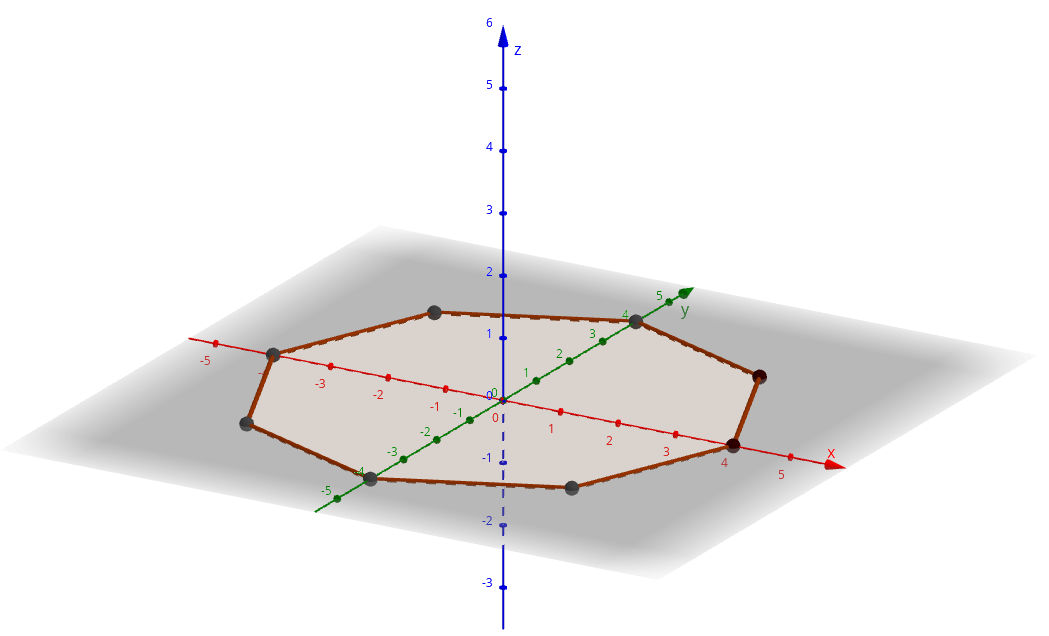
\includegraphics[width = 5cm]{images/octagon.png}
\end{center}
\end{figure}
\pause
Representation \(\rho: D_{2n} \to \GL (\R^3)\) with 
\begin{itemize}
\item \(\rho(a)\) as rotation about the \(Z\)-axis
\item \(\rho(b)\) as a rotation about a suitable axis in the \(XY\)-plane
\end{itemize}
\end{example}
\end{frame}

\note{
Slide with the example: Raphael
}

\begin{frame}
\frametitle{Invariant subspaces, Irreducibility}
\begin{definition}
Let \(V\) be a representation and \(U \subseteq V\) a subspace. \(U\) is an \textbf{invariant subspace} if \(gu \in U\) for \(\forall u\in U, g \in G\).
\end{definition}
\pause
\begin{example}
\begin{figure}[h]
\begin{center}
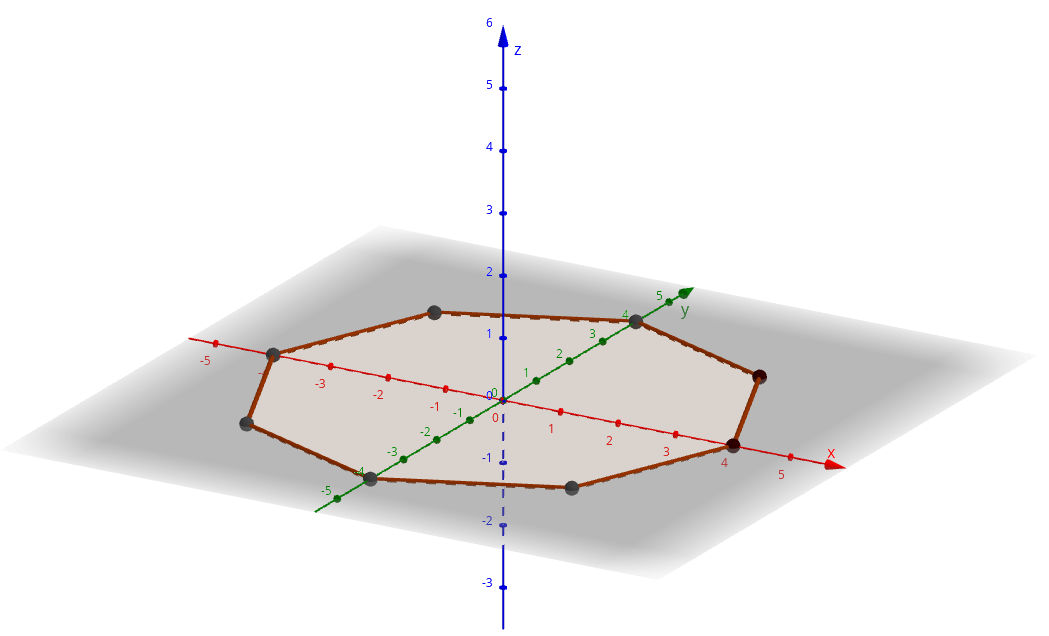
\includegraphics[width = 3cm]{images/octagon.png}
\end{center}
\end{figure}
\pause
The \(XY\)-Plane is an invariant subspace.
\end{example}
\end{frame}

\note{
Invariant Subspaces, Irreducibility: Paul
-> The Z-axis is an invariant subspace as well (and a complement!)
}

\begin{frame}
\frametitle{Irreducibility, Representation Homomorphisms}
\begin{definition}
A representation \(V\) is \textbf{irreducible} provided \(V \neq 0\) and the only invariant subspaces are 0 and \(V\).
\end{definition}
\pause
\begin{definition}
For representations \(V\) and \(W\), a \textbf{homomorphism} is a linear map \(\theta: V\to W\) with \(\theta(gv) = g\theta(v)\) for \(\forall g\in G, v\in V\).
\end{definition}
\pause
\begin{itemize}
\item \(\Img (\theta)\) and \(\Ker (\theta)\) are invariant subspaces
\item If \(V\) and \(W\) are irreducible, then \(\theta: V \to W\) is 0 or bijective.
\end{itemize}
\end{frame}

\note{
Irreducibility, Representation Homomorphisms: Raphael
The following section: Paul
}

\section{Finite abelian groups}
\begin{frame}
\frametitle{Main theorem formalized in this project}
This theorem is listed on the \enquote{Missing undergraduate mathematics in mathlib}-page.
\pause
\begin{theorem}
Let \(G\) be a finite abelian group.\\
Let \(V\) be a non-null vector space over an algebraically closed field \(k\).\\
Let \(\rho: G \to \GL (V)\) be a representation.\\
\pause
\vspace{1cm}
Then \(\rho\) is irreducible if and only if \(\dim_k(V) = 1\).
\end{theorem}
\end{frame}

\begin{frame}
\frametitle{Proof of the theorem}
\begin{theorem}
\(\rho\) is irreducible if and only if \(\dim_k(V) = 1\).
\end{theorem}
\pause
\enquote{\(\Leftarrow\)} is trivial.\\
\pause
For \enquote{\(\Rightarrow\)}, we use the following two lemmas:
\begin{lemma}
For all \(g \in G\), \(\rho(g)\) is a Representation Endomorphism.
\end{lemma}
\pause
\begin{lemma}
Every Representation Endomorphism is given by multiplication with a scalar.
\end{lemma}
\end{frame}

\note{
\begin{itemize}
\item in the first lemma, we use the fact that \(G\) is abelian
\item the second lemma is a corollary of Schur's lemma
\item There are versions of Schur's lemma in Mathlib, but we proved it from scratch
\item in the second lemma, we use that the field is algebraically closed
\end{itemize}
}

\begin{frame}
\frametitle{Proof of the theorem}
With these two lemmas, we can prove the following fact:
\begin{lemma}
Every one-dimensional subspace of \(V\) is an invariant subspace.
\end{lemma}
\pause
Now, we can use proof by contradiction:
\pause
\begin{enumerate}
\item Assume \(\dim (V) > 1\).
\pause
\item Then, \(V\) has a proper subspace with dimension 1.
\pause
\item So \(V\) has a proper invariant subspace.
\pause
\item This is a contradiction to the irreducibility of \(V\).
\end{enumerate}
\end{frame}

\note{
This section is followed by Paul showing the code: General structure, multiple files, definitions...
}

\section{Formalization}
\begin{frame}[fragile]
\frametitle{Representations in Mathlib}
Representations are already defined in Mathlib:
\begin{lstlisting}
abbrev Representation :=
  G →* V →ₗ[k] V

end
\end{lstlisting}
\pause
Apart from that, the definitions introduced in the beginning of this presentation are missing in Mathlib.
\end{frame}

\note{
Representations in Mathlib: Raphael
}

\begin{frame}[fragile]
\frametitle{Definitions}
\begin{lstlisting}
/-- A predicate for a subspace being invariant -/
def IsInvariantSubspace {k G V : Type*} [CommSemiring k] [Monoid G] [AddCommMonoid V] [Module k V]
  (U : Submodule k V) (ρ : Representation k G V) :=
  ∀ g : G, ∀ u : U, ρ g u ∈ U

/-- defines degree of a representation as rank of its module -/
def degree {k G V : Type*} [CommSemiring k] [Monoid G] [AddCommMonoid V] [Module k V]
  (ρ : Representation k G V) : Cardinal := (Module.rank k V)
\end{lstlisting}
\end{frame}

\note{
Definitions: Paul
\begin{itemize}
\item Left out irreducibilty for space
\item Commentary about class inference
\end{itemize}
}

\begin{frame}[fragile]
\frametitle{Representation Homomorphisms}
\begin{definition}
For representations \(V\) and \(W\), a \textbf{homomorphism} is a linear map \(\theta: V\to W\) with \(\theta(gv) = g\theta(v)\) for \(\forall g\in G, v\in V\).
\end{definition}
\begin{lstlisting}
/-- Definition of Homomorhpisms between Representations -/
@[ext] class RepresentationHom {k G V W : Type*} [CommSemiring k] [Monoid G] [AddCommMonoid V] [Module k V] [AddCommMonoid W] [Module k W]
  (ρ : Representation k G V) (ψ : Representation k G W) extends LinearMap (RingHom.id k) V W where
  reprStructure : ∀ g : G, ∀ v : V, toLinearMap (ρ g v) = ψ g (toLinearMap v)
\end{lstlisting}
\end{frame}

\note{Representation Homomorphisms: Raphael
- say that this definition adapts Mathlib definitions of maps
- say that we tried to match the Mathlib style in other definitions as well}

\begin{frame}[fragile]
\frametitle{Coercions}
\begin{lstlisting}
/-- Coercions of RepresentationHom to Function and Linear Map-/
instance {k G V W : Type*} [CommSemiring k] [Monoid G] [AddCommMonoid V] [Module k V] [AddCommMonoid W] [Module k W] {ρ : Representation k G V} {ψ : Representation k G W} : CoeFun (RepresentationHom ρ ψ) (fun _ ↦ V →ₗ[k] W) where
  coe := by
    intro θ
    use ⟨θ.toFun, ?_⟩
    simp; intro x y; simp
\end{lstlisting}
\end{frame}

\note{
Coercions: Paul
}

\begin{frame}[fragile]
\frametitle{Registering Instances}
\begin{lemma}
For all \(g \in G\), \(\rho(g)\) is a Representation Endomorphism.
\end{lemma}
\begin{lstlisting}
instance repr_yields_reprHom_commMonoid {k G V : Type*} [CommSemiring k] [CommMonoid G] [AddCommMonoid V] [Module k V]
  (ρ : Representation k G V) (g : G) : (RepresentationHom ρ ρ) where
  toFun := ρ g
  map_add' := by intro x y; simp
  map_smul' := by intro m x; simp
  reprStructure := sorry
\end{lstlisting}
\end{frame}

\note{
Registering Instances: Raphael
The following section: Raphael
\begin{itemize}
\item Code in place of sorry is left out for space
\item The rest of the code is using these definitions => probably not that interesting
\end{itemize}
}

\section{Mathlib}
\begin{frame}
\frametitle{Representation Theory in Mathlib}
Things already contained in Mathlib:
\begin{itemize}
\item Definition of Representations, basic properties, duality
\item Category Theory
\item Characters
\end{itemize}
\pause
Things not contained in Mathlib:
\begin{itemize}
\item Subrepresentations, Homomorphisms, Irreducibility
\item Direct sums, reducibility, Maschke for Representations
\item \ldots
\end{itemize}
\end{frame}

\note{
Irreducibilty is contained in category theory
}

\begin{frame}
\frametitle{Two views on Representations}
A representation \((V, \rho)\) can be \enquote{translated} to a module over a \(k\)-algebra \(kG\):\\
\pause
Take a \(k\)-module with basis \(\{g\vert g\in G\}\) and multiplication
\begin{equation*}
\left(\sum_{g\in G}\lambda_g g\right)\cdot \left(\sum_{h\in G}\mu_h h\right) = \sum_{g,h\in G} \lambda_g\mu_h (gh)
\end{equation*}
\pause
with action
\begin{equation*}
kG\times V\to V, \left(\sum_{g\in G}\lambda_gg, v\right) \mapsto \sum_{g\in G}\lambda_g(gv).
\end{equation*}
\end{frame}

\note{
Of course, the translation works the other way as well!
}

\begin{frame}[fragile]
\frametitle{The translation in Mathlib}
Irreducibility of representations translates to simplicity of modules.\\
\pause
Things like the theorem of Maschke are not formulated for \verb+Representation+s, but for modules over algebras.\\
\pause
\vspace{1cm}
\begin{itemize}
\item \verb+Representation.asModule+ translates \verb+Representation+ to algebra
\item \verb+Representation.ofModule+ translates algebra to \verb+Representation+
\end{itemize}
\end{frame}

\note{
The following section and the outro: Paul
}

\section{Future work}
\begin{frame}
\frametitle{Future work}
\begin{itemize}
\pause
\item Connect Algebras and Representations: Irreducibility, \ldots
\pause
\item Formulate theorem of Maschke for Representations
\pause
\item Add additional theorems about Representation Theory of finite groups
\item \ldots
\end{itemize}
\end{frame}

\note{
The thing with Maschke is declared as Future Work in Mathlib
}

\begin{frame}
\begin{center}
\huge Questions?
\end{center}
\end{frame}

\end{document}